% Solution: Tadelis (2013) Exercise 7.4 "Centipedes". Input by \solitem.
% New in the 50-item list. Check: check_B_L03.py.
\begin{exsol}{Tadelis Exercise 7.4}{148}{Exam}{3}
\asked In the four-move grab/share game with a pot of \$6 growing by $\frac32$: (a) tree and type
of information; (b) terminal nodes and information sets; (c) pure strategies; (d) Nash equilibria
and how many outcomes they support; (e) the same when sharing at the last node splits the pot
equally.

\method Tree, information sets and perfect information (Lecture~3, slides~20--24; Tadelis
\S7.1, pp.~133--136); strategies as complete plans (slide~25; Def.~7.4, p.~138); the normal form
and its Nash equilibria (Tadelis \S7.2.3, pp.~142--145); backward induction to identify the
sequentially rational one (slides~29--30; Tadelis \S8.1, pp.~152--153; the centipede game itself is
Tadelis \S8.3.1, pp.~159--160). Nash equilibrium constrains play only on the path, so the outcome
argument proceeds forward from the last node that is reached with positive probability.

\solution
\textbf{Pot and payoffs.} The pot before move $k = 1, 2, 3, 4$ is $6 \cdot (\frac32)^{k-1}$:
$6,\ 9,\ \frac{27}{2},\ \frac{81}{4}$; after a share at move~4 it is $\frac{243}{8}$. A grab gives
the mover $\frac23$ of the current pot and the other player $\frac13$. Payoffs $(u_1,u_2)$:
\begin{center}
\begin{tabular}{lccc}
\toprule
Terminal history & pot & $u_1$ & $u_2$ \\
\midrule
$G$ (1 grabs at move 1) & $6$ & $4$ & $2$ \\
$SG$ (2 grabs at move 2) & $9$ & $3$ & $6$ \\
$SSG$ (1 grabs at move 3) & $\frac{27}{2}$ & $9$ & $\frac92$ \\
$SSSG$ (2 grabs at move 4) & $\frac{81}{4}$ & $\frac{27}{4}$ & $\frac{27}{2}$ \\
$SSSS$ (2 shares at move 4) & $\frac{243}{8}$ & $\frac{81}{4}$ & $\frac{81}{8}$ \\
\bottomrule
\end{tabular}
\end{center}

\textbf{(a) Tree.} Perfect information: every information set is a single node.
\begin{center}
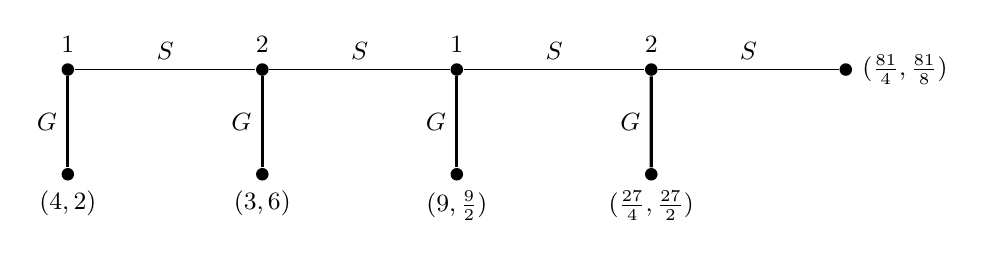
\begin{tikzpicture}[scale=0.95,dot/.style={circle,fill,inner sep=1.6pt},
  every node/.style={font=\small}]
  \foreach \i/\pl in {0/1,1/2,2/1,3/2} {
    \node[dot,label=above:{\pl}] (n\i) at (2.6*\i,0) {};
  }
  \node[dot,label=right:{$(\frac{81}{4},\frac{81}{8})$}] (end) at (10.4,0) {};
  \draw (n0) -- node[above] {$S$} (n1);
  \draw (n1) -- node[above] {$S$} (n2);
  \draw (n2) -- node[above] {$S$} (n3);
  \draw (n3) -- node[above] {$S$} (end);
  \foreach \i/\pay in {0/{$(4,2)$},1/{$(3,6)$},2/{$(9,\frac92)$},3/{$(\frac{27}{4},\frac{27}{2})$}} {
    \node[dot,label=below:{\pay}] (g\i) at (2.6*\i,-1.4) {};
    \draw[very thick] (n\i) -- node[left] {$G$} (g\i);
  }
\end{tikzpicture}\\[2pt]
{\footnotesize Thick branches = backward-induction choices (part (d)).}
\end{center}

\textbf{(b) Counts.} Terminal nodes: \textbf{5} (four grabs and the final share). Information sets:
\textbf{4}, two per player (moves 1 and 3 for player~1, moves 2 and 4 for player~2).

\textbf{(c) Pure strategies.} Each player has 2 information sets with 2 actions: $2^2 = 4$ pure
strategies each. Write $s_1 = (\text{move 1}, \text{move 3})$ and $s_2 = (\text{move 2},
\text{move 4})$: $S_1 = S_2 = \{GG, GS, SG, SS\}$.

\textbf{(d) Nash equilibria.} \emph{Backward induction first.} Move~4: player~2 grabs
($\frac{27}{2} > \frac{81}{8}$). Move~3: player~1 grabs ($9 > \frac{27}{4}$). Move~2: player~2
grabs ($6 > \frac92$). Move~1: player~1 grabs ($4 > 3$). SPE $= (GG, GG)$, payoffs $(4, 2)$.

\emph{Normal form} (rows player~1, columns player~2):
\begin{center}
\begin{tabular}{r|c|c|c|c|}
\multicolumn{1}{r}{} & \multicolumn{1}{c}{$GG$} & \multicolumn{1}{c}{$GS$} &
\multicolumn{1}{c}{$SG$} & \multicolumn{1}{c}{$SS$}\\ \cline{2-5}
$GG$ & $\br{4},\ \br{2}$ & $\br{4},\ \br{2}$ & $4,\ \br{2}$ & $4,\ \br{2}$ \\ \cline{2-5}
$GS$ & $\br{4},\ \br{2}$ & $\br{4},\ \br{2}$ & $4,\ \br{2}$ & $4,\ \br{2}$ \\ \cline{2-5}
$SG$ & $3,\ \br{6}$ & $3,\ \br{6}$ & $\br{9},\ \frac92$ & $9,\ \frac92$ \\ \cline{2-5}
$SS$ & $3,\ 6$ & $3,\ 6$ & $\frac{27}{4},\ \br{\frac{27}{2}}$ & $\br{\frac{81}{4}},\ \frac{81}{8}$ \\ \cline{2-5}
\end{tabular}
\end{center}
(Underlined payoffs are best replies. Outside the top-left block no cell has both payoffs
underlined: in row $SS$ player~2's best reply is $SG$, against which player~1 prefers $SG$, against
which player~2 prefers to grab at move~2.) The \textbf{pure Nash equilibria} are the
four profiles $\{GG, GS\} \times \{GG, GS\}$: player~1 grabs at once and player~2 plans to grab
at move~2; what either plans at the later, unreached node is free. Every one gives the outcome
$G$ with $(4,2)$.

\emph{Mixed equilibria: still one outcome.} Work forward along a Nash equilibrium, using that
every node reached with positive probability must be played optimally given what follows.
(i) If move~4 is reached, player~2 grabs there ($\frac{27}{2} > \frac{81}{8}$). (ii) So if move~3 is
reached, sharing gives player~1 $\frac{27}{4}$ against $9$ from grabbing: he grabs, and move~4 is
never reached. (iii) So if move~2 is reached, sharing gives player~2 $\frac92$ against $6$ from
grabbing: she grabs, and move~3 is never reached. (iv) So sharing at move~1 gives player~1
$3 < 4$: he grabs. Hence \textbf{every} Nash equilibrium has player~1 grabbing at move~1:
\textbf{one outcome}, $(4,2)$. The mixed equilibria differ only off
the path. With $g = \Pr_2(G \text{ at move 2})$ and $h = \Pr_2(G \text{ at move 4})$, player~1's best
deviation (share, then the better of grabbing for 9 or sharing for
$M = \max\{9,\ \frac{27}{4}h + \frac{81}{4}(1-h)\}$) must not beat 4:
\[
  3g + M(1-g) \le 4 \iff g \ge 1 - \frac{1}{M - 3},
\]
e.g.\ $g \ge \frac56$ if $h = 1$ and $g \ge \frac{65}{69}$ if $h = 0$.

\textbf{(e) Equal split at the end.} Sharing at move~4 now gives each player
$\frac12\cdot\frac{243}{8} = \frac{243}{16} \approx 15.19$. Backward induction: move~4: share
($\frac{243}{16} > \frac{27}{2} = \frac{216}{16}$); move~3: share ($\frac{243}{16} > 9$); move~2:
share ($\frac{243}{16} > 6$); move~1: share ($\frac{243}{16} > 4$). SPE $= (SS, SS)$ with payoffs
$(\frac{243}{16}, \frac{243}{16})$. The answer to (d) changes: the pure Nash equilibria are now
$(SS, SS)$ and, as before, the four profiles $\{GG,GS\}\times\{GG,GS\}$ (player~2's plan to grab at
move~2 still deters player~1, and it is never tested). So \textbf{two outcomes} are supported: grab
at once, $(4,2)$, and share to the end, $(\frac{243}{16}, \frac{243}{16})$. Grabbing at move 2, 3 or
4 is never an equilibrium outcome: the grabber at move~4 would rather share, the grabber at move~3
would be pre-empted at move~2 (player~2 compares $6$ with $\frac92$), and a grab at move~2 leaves
player~1 with $3 < 4$.

\interp With the original split the mover at the last node always grabs, and the anticipation
unravels cooperation back to the first move: the pot that could have grown to $\$30$ is
grabbed at $\$6$. Changing only the \emph{last} node's rule (an equal split) turns the last mover
into someone who wants to continue, and the whole chain of reasoning reverses. Credibility at the
end of the game drives behavior at the start, the backward-induction lesson of Lecture~3 and the
reason why commitments that change the final payoffs (Lecture~4, slide~11) are so powerful.

\verify \texttt{check\_B\_L03.py} builds the tree with exact fractions (pots
$6, 9, \frac{27}{2}, \frac{81}{4}, \frac{243}{8}$), runs backward induction (unique solution:
grab, $(4,2)$), builds the $4\times4$ normal form and finds exactly the four pure Nash equilibria,
all with outcome $(4,2)$; it checks the bound on $g$ at $h \in \{0, \frac12, 1\}$ on both sides
($\frac56$, $\frac{65}{69}$); for (e) it finds the SPE all-share with
$(\frac{243}{16}, \frac{243}{16})$ and the five pure Nash equilibria with two outcomes. Output line:
\texttt{tadelis-7-4: (d) 4 pure NE, one outcome (4, 2); (e) SPE all-share 243/16 each; NE outcomes
2}. Tadelis prints no answer.

\mistakes
\begin{itemize}
  \item Answering ``one Nash equilibrium'' in (d): there are four pure ones (and a continuum of
  mixed ones); it is the \emph{outcome} that is unique.
  \item Misreading the last-node rule in (d): if player~2 shares at move~4 she gets only $\frac13$
  of the pot, $\frac{81}{8} < \frac{27}{2}$, so she grabs.
  \item In (e), concluding that sharing is the only equilibrium outcome: the immediate grab is still
  a (non-subgame-perfect) Nash equilibrium.
\end{itemize}

\answer{(a) Tree above; perfect information. (b) 5 terminal nodes; 4 information sets (2 each).
(c) 4 pure strategies each: $GG, GS, SG, SS$. (d) Pure Nash equilibria: $\{GG,GS\}\times\{GG,GS\}$;
every Nash equilibrium (mixed ones too) has player~1 grabbing at once: one outcome, $(4,2)$; SPE
$(GG,GG)$. (e) Yes: SPE $(SS,SS)$ with $(\frac{243}{16},\frac{243}{16})$; pure Nash equilibria
$(SS,SS)$ and $\{GG,GS\}\times\{GG,GS\}$; two outcomes.}
\end{exsol}
